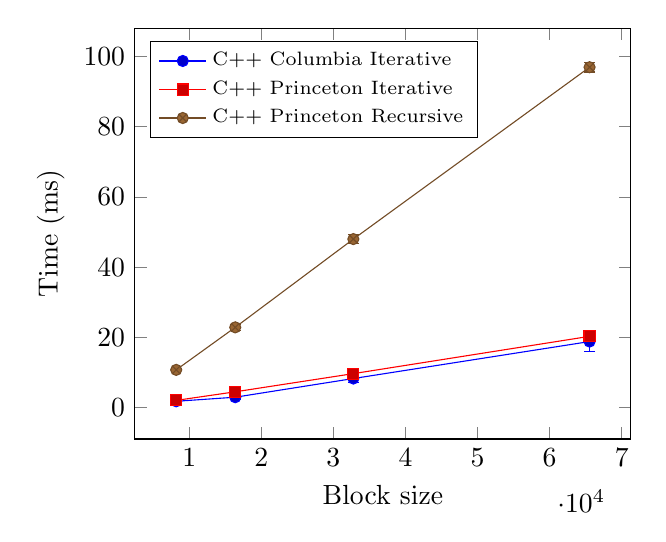
\begin{tikzpicture}
\begin{axis}[xlabel={Block size},ylabel={Time (ms)},width=0.65\linewidth,legend pos=north west,scaled y ticks = false,legend cell align=left,legend style={font=\scriptsize}]
\addplot+[error bars/.cd, y dir=both,y explicit] coordinates {
(8192, 1.8030) +- (0.9841, 0.9841)
(16384, 2.9629) +- (0.6687, 0.6687)
(32768, 8.2847) +- (1.2061, 1.2061)
(65536, 18.8158) +- (2.8032, 2.8032)
};
\addplot+[error bars/.cd, y dir=both,y explicit] coordinates {
(8192, 2.0605) +- (0.0561, 0.0561)
(16384, 4.5027) +- (0.1737, 0.1737)
(32768, 9.6797) +- (0.6568, 0.6568)
(65536, 20.3049) +- (1.7691, 1.7691)
};
\addplot+[error bars/.cd, y dir=both,y explicit] coordinates {
(8192, 10.7496) +- (0.2605, 0.2605)
(16384, 22.8640) +- (0.8917, 0.8917)
(32768, 48.0022) +- (1.2536, 1.2536)
(65536, 96.9572) +- (1.3564, 1.3564)
};
\legend{C++ Columbia Iterative , C++ Princeton Iterative , C++ Princeton Recursive}
\end{axis}
\end{tikzpicture}
